\documentclass[border=3pt]{standalone}
% Preâmbulo compartilhado pelos diagramas TikZ da aula 5 de IHC (Processos de Design)
\usepackage[T1]{fontenc}
\usepackage[utf8]{inputenc}
\usepackage{lmodern}
\usepackage{amsmath}
\usepackage{xcolor}
\usepackage{tikz}
\usetikzlibrary{arrows.meta,angles,quotes,decorations.pathmorphing,calc,
                positioning,shapes.geometric,shapes.misc,backgrounds,fit,
                math}

% Paleta (mesma dos SVGs originais)
% Paleta da disciplina de IHC: acento roxo (#755099), da capa do livro.
% (o nome "dblue" é mantido para não alterar todos os diagramas)
\definecolor{dblue}{HTML}{755099}
\definecolor{dorange}{HTML}{B3541E}
\definecolor{dgreen}{HTML}{4A7C59}
\definecolor{dred}{HTML}{9C4B4B}
\definecolor{dcream}{HTML}{F4F1EA}
\definecolor{dshade}{HTML}{DDD7C9}

% Função gaussiana (não normalizada por padrão de escala visual)
\pgfmathdeclarefunction{gauss}{3}{%
  \pgfmathparse{1/(#3*sqrt(2*pi))*exp(-((#1-#2)^2)/(2*#3^2))}%
}

% Estilos comuns (prefixo d... para não colidir com chaves internas do pgf)
\tikzset{
  >={Stealth[length=2mm]},
  dguide/.style={gray!55, dashed, line width=0.4pt},
  daxis/.style={gray!60, line width=0.7pt, ->},
  dbody/.style={fill=black!3, draw=black!80, line width=1pt},
  dacc/.style={draw=dblue, line width=1pt},
  dlbl/.style={black!55, font=\small},
  dsub/.style={black!45, font=\footnotesize},
  dstate/.style={circle, draw=black!80, fill=dcream, line width=1pt,
                 minimum size=17mm, font=\large, inner sep=1pt},
  dobs/.style={circle, draw=black!80, fill=dshade, line width=1pt,
               minimum size=14mm, font=\large, inner sep=1pt},
  dbox/.style={rounded corners=2pt, draw=black!80, fill=dcream, line width=1pt,
               align=center, inner sep=6pt},
  dop/.style={circle, draw=black!80, fill=white, line width=1pt,
              minimum size=6mm, inner sep=0pt, font=\small},
  dtrans/.style={->, dblue, line width=1pt},
  dmeas/.style={->, dorange, line width=1pt},
  dcurve/.style={line width=1pt, dblue},
  dcurveb/.style={line width=1.4pt, dorange},
}

\begin{document}
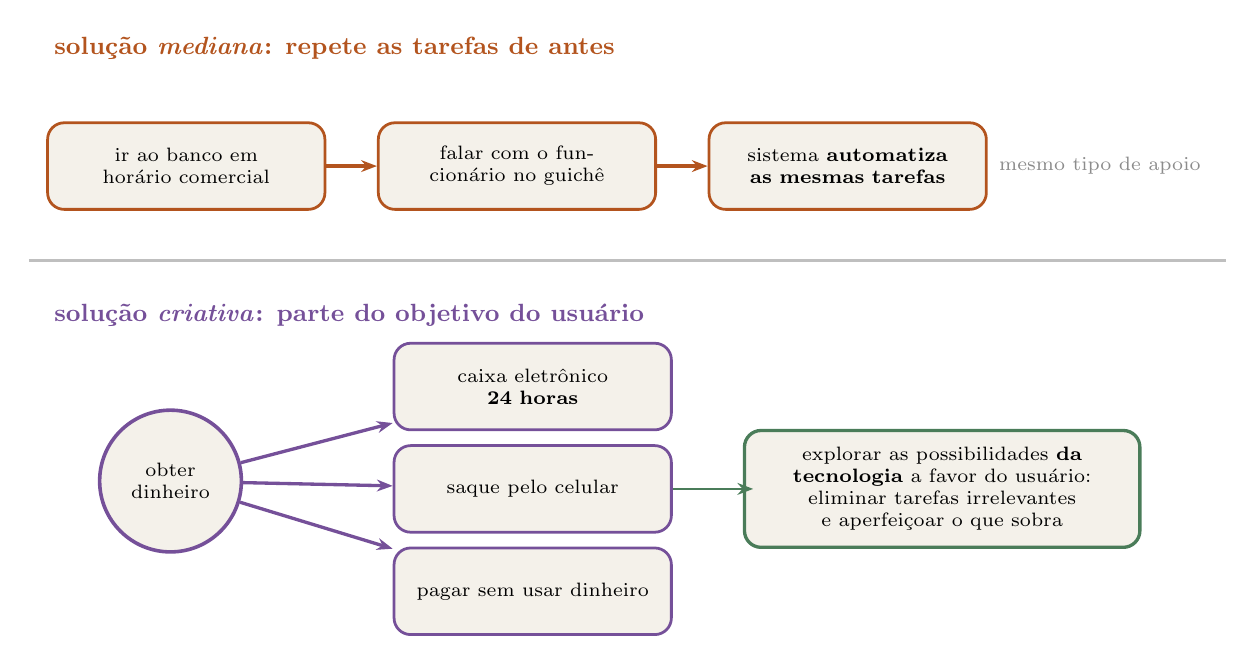
\begin{tikzpicture}[x=1cm,y=1cm,
   t/.style={dbox, rounded corners=6pt, text width=3.1cm, minimum height=1.1cm, font=\scriptsize}]

  \node[font=\small\bfseries, dorange, anchor=west] at (0,3.7) {solução \textit{mediana}: repete as tarefas de antes};
  \node[t, draw=dorange] (a1) at (1.8,2.2) {ir ao banco em horário comercial};
  \node[t, draw=dorange] (a2) at (6.0,2.2) {falar com o funcionário no guichê};
  \node[t, draw=dorange] (a3) at (10.2,2.2) {sistema \textbf{automatiza as mesmas tarefas}};
  \draw[->, dorange, line width=1.2pt] (a1) -- (a2); \draw[->, dorange, line width=1.2pt] (a2) -- (a3);
  \node[dsub, font=\scriptsize, anchor=west] at (12.0,2.2) {mesmo tipo de apoio};

  \draw[black!25, line width=0.8pt] (-0.2,1.0) -- (15.0,1.0);

  \node[font=\small\bfseries, dblue, anchor=west] at (0,0.3) {solução \textit{criativa}: parte do \textbf{objetivo} do usuário};
  \node[dstate, minimum size=18mm, font=\scriptsize, text width=1.6cm, align=center, draw=dblue, line width=1.3pt] (o) at (1.6,-1.8) {obter dinheiro};
  \node[t, draw=dblue] (b1) at (6.2,-0.6) {caixa eletrônico \textbf{24 horas}};
  \node[t, draw=dblue] (b2) at (6.2,-1.9) {saque pelo celular};
  \node[t, draw=dblue] (b3) at (6.2,-3.2) {pagar sem usar dinheiro};
  \draw[->, dblue, line width=1.2pt] (o) -- (b1); \draw[->, dblue, line width=1.2pt] (o) -- (b2); \draw[->, dblue, line width=1.2pt] (o) -- (b3);
  \node[dbox, draw=dgreen, line width=1.2pt, text width=4.6cm, font=\scriptsize, rounded corners=6pt] at (11.4,-1.9) {explorar as possibilidades \textbf{da tecnologia} a favor do usuário: eliminar tarefas irrelevantes e aperfeiçoar o que sobra};
  \draw[->, dgreen, line width=1pt] (b2.east) -- (9.0,-1.9);

\end{tikzpicture}
\end{document}
